% vim:spell spelllang=sk
%\subsection{Image processing}
\section{Image processing}

Táto kapitola bude venovaná spracovaniu obrazovej informácie a~ako sa
pri tom dá využiť Fourierova transformácia. Ukážeme si dôležitosť
magnitúdy a~fázy, rýchle hľadanie patternu rovnakej
veľkosti a~orientácie. O~digitálnych filtroch a~ich aplikácii
na filtrovanie obrázkov sme už písali v~predchádzajúcej kapitole 
a~preto tu uvedieme len veci netýkajúce sa úplne priamo filtrov.

%\subsubsection{Fourierova transformácia - fáza a magnitúda}
\subsection{Fourierova transformácia - fáza a magnitúda}
Zatiaľ nikde v~tomto texte sme nespomínali previazanosť fázy 
a~magnitúdy u~Fourierovej transformácie. Je preto normálne sa pýtať, či
majú rovnakú váhu na vzniku výsledného obrazu. Odpoveď je prekvapivá -
nie. Fáza sa omnoho výraznejšie podieľa na výsledných črtách, ako
magnitúda. Túto skutočnosť prezentujeme na ilustrácii
\ref{fig:image_phase_magnitude}. Môžeme pozorovať, že obrázok síce
kompletnou zmenou magnitúdy stratí textúru, bude v~ňom šum, ale
základné črty si predsa len zachová. Objekt je rozpoznateľný aj po
takých výrazných zmenách magnitúdy, ako sú zmena na konštantu, či
výmena s~iným obrázkom. Naopak, posledné dva obrázky ukazujú skutočnosť,
že položením konštantnej fázy úplne zrušíme vizuálnu informáciu.
Zaujímavým efektom, ktorý možno pozorovať je príspevok strechy prvého
obrázku k~druhému. Strecha totiž obsahuje pomerne výraznú
hranu-diskontinuitu natočenú o~45~stupňov a~prispieva tak výrazne
k~rovnako orientovanému šumu.

%%% {{{ fig:mix_phase_magnitude
\begin{figure}[htp]
    \def\path{obrazky/informatika/image_processing/mix_phase_magnitude/}
 \centering
  \subfigure[Fáza 1, Magnitúda 1]{
    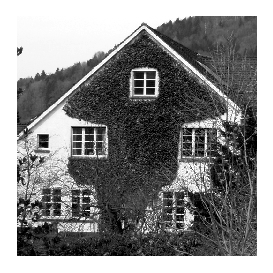
\includegraphics{\path/p1m1}
  }
  \subfigure[Fáza 1, Magnitúda 2]{
    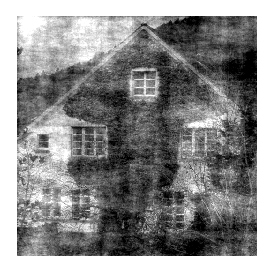
\includegraphics{\path/p1m2}
  }
  \subfigure[Fáza 1, konšt. Magnitúda]{
    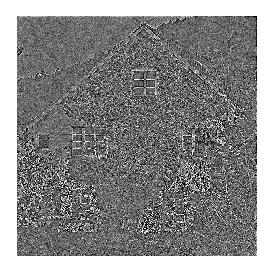
\includegraphics{\path/p1mc}
  }
  \subfigure[Fáza 2, Magnitúda 1]{
    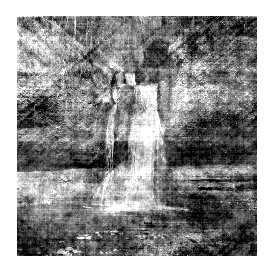
\includegraphics{\path/p2m1}
  }
  \subfigure[Fáza 2, Magnitúda 2]{
    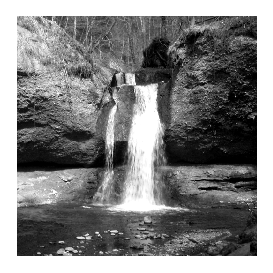
\includegraphics{\path/p2m2}
  }
  \subfigure[Fáza 2, konšt. Magnitúda]{
    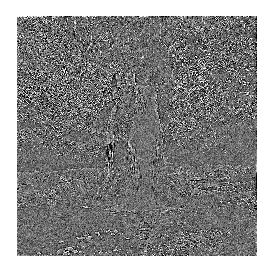
\includegraphics{\path/p2mc}
  }
  \subfigure[Konšt. fáza, Magnitúda 1]{
    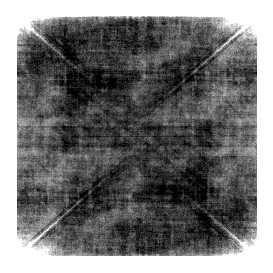
\includegraphics{\path/pcm1}
  }
  \subfigure[Konšt. fáza, Magnitúda 2]{
    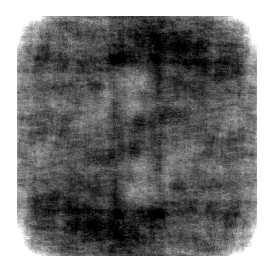
\includegraphics{\path/pcm2}
  }
    \caption{Porovnanie dôležitosti fázy a magnitúdy}
    \label{fig:image_phase_magnitude}
\end{figure}
%% }}}
\smalltodo{Undefine path}
Dôležitosť fázy ale nekončí len pri obrázkoch. V~elektronickej verzii
tohoto diela sa čitateľ môže presvedčiť o~tom istom závere na audio
súboroch.


%\subsubsection{Hľadanie patternov}
\subsection{Hľadanie patternov}
Jednou z~nečakaných aplikácii konvolúcie je aj takzvaný korelačný
filter. Korelácia sa používa na identifikáciu lineárnej závislosti.
Začneme štandardnou definíciou korelácie zo štatistiky
\begin{definicia}[Korelácia]
  Koreláciou dvoch nenulových postupností $x,y$ nazveme číslo
  \begin{equation*}
    r_{x,y} = \frac{E(xy)-E(x)E(y)}{D(x)D(y)} =
        \frac{\displaystyle
            n \sum_{i=0}^{n-1} x_i y_i - \sum_{i=0}^{n-1} x_i
            \sum_{i=0}^{n-1} y_i}{\displaystyle
        \sqrt{n \sum_{i=0}^{n-1} x_i^2 - 
            \left(\sum_{i=0}^{n-1}x_i\right)^2}
        \sqrt{n \sum_{i=0}^{n-1} y_i^2 - 
            \left(\sum_{i=0}^{n-1} y_i\right)^2}}
  \end{equation*}
\end{definicia}
Korelácia popisuje mieru lineárnej závislosti oboch postupností.
Použitím Cauchy-Schwarzovej nerovnosti (veta
\ref{veta:cauchy_schwarz}) pomerne jednoducho dostávame
nerovnosť $|r_{x,y}| \le 1$ s~rovnosťou nastávajúcou práve v~prípade
lineárnej závislosti. Zjednodušene povedané, čím je väčšia korelácia
(v~absolútnej hodnote), tým viac sa na seba dané postupnosti podobajú,
zoberúc do úvahy ich relatívne škálovanie. Korelácia je preto veľmi
vhodný nástroj v~spracovávaní signálu na hľadanie známej vzorky 
v~danom signáli. Musíme ale nájsť efektívnu cestu ako ju rýchlo počítať.
\begin{definicia}[Nenormalizovaná korelácia]
    Nenormalizovanou koreláciou nazveme hodnotu
    \begin{equation*}
        r'_{x,y} = \sum_{i=0}^{n-1} x_i y_i
    \end{equation*}
\end{definicia}
Čakajú nás dve podúlohy - rýchle počítanie nenormalizovanej korelácie 
a~následne efektívny prepočet na normalizovanú koreláciu.
Aby sme spresnili úlohu - na vstupe máme známy pattern $y_0,\dots,y_{n-1}$
dĺžky $n$ a~signál (pravdepodobne) väčšej dĺžky $x_0,\dots, x_{m-1}$.
Chceme vypočítať postupne
$r_{x_0\dots x_{n-1},y}, r_{x_1\dots x_n,y}, r_{x_2\dots x_{n+1},y},\dots$.
Pretože zameraním celej tento práce je Fourierova transformácia,
dostávame drobný hint. Konkrétne, poznáme podobnú rovnicu - konvolúciu.
Skutočne, konvolúcia a korelácia sú jedna a~tá istá operácia, ak
"otočíme" postupnosť $y$.
Formálne
\begin{lema}
    Nech $x'$ je postupnosť $x$ rozšírená nulami na dĺžku $n+m$.
    Nech $y'$ je postupnosť dĺžky $n+m$ definovaná nasledovne
        $y'=[y_0, \textit{$m$ krát }0, y_{n-1}, y_{n-2}, \dots, y_2,
        y_1]$.
    Potom $r_{x_i,y} = conv(x,y)_i$ kde $conv$ označuje (necyklickú)
    konvolúciu.
\end{lema}
\begin{dokaz}
    Dôkaz je podobný dôkazu lemy \ref{lema:filter_konvolucia}
\end{dokaz}
Nenormalizovanú koreláciu vieme preto rýchlo vypočítať pomocou
Fourierovej transformácie. Ostáva určiť, ako ju efektívne prepočítať
na normalizovanú.
Prvým krokom bude "normalizácia" $y$ vzorcom $y' = y-E(y)$, inak povedané,
odčítanie priemeru. Táto transformácia nezmení hodnotu korelácie, ako
sa môžeme presvedčiť
\begin{align*}
    E(x (y-E(y))) &= E(x y - x E(y)) = E(xy) - E(x E(y)) = E(xy) -
    E(x)E(y) \\
    D(y - E(y)) &= D(y)
\end{align*}
V~čitateli ostala nenormalizovaná korelácia $x,y'$, v~menovateli
konštantná hodnota $D(y)$ ľahko vypočítateľná na začiatku a $D(x)=
D([x_i,x_{i+1},\dots,x_{i+n-1}])$,
ktorá sa mení. Našťastie, táto hodnota sa dá efektívne počítať. 
V~jednom rozmere napríklad nasledovne - pamätáme si sumu posledných $n$
hodnôt a~ich druhých mocnín a~keď sa posúvame o~hodnotu vpravo,
pripočítame
nový člen a~odpočítame hodnotu toho, ktorý "vypadol" z~postupnosti. 
V~dvoch (a~viacerých) rozmeroch sa dajú predpočítať prefixové sumy 
v~lineárnom čase s~následnou otázkou na sumu obdĺžnika v~konštantnom
čase.

Po vyriešení algoritmickej strany problému sa zamyslíme na čo je
korelácia vhodná. Jedno teoretické použitie je znázornené na obrázku
\ref{fig:korelacia}. Ide o~stroj overujíci pravosť bankovky 
a~hľadajúci známe znaky. Na obrázku je znázornený známy pattern, ktorý
chceme identifikovať v~rámci obrázku, symbol eura. Vedľa neho je
znázornená korelácia daných dvoch vzorov, ukazujúca maximum presne na
polohe hľadaného symbolu. Stroj takto môže identifikovať viacero
symbolov, porovnať ich pozície a~kvalitu korelácie a~identifikovať
bankovku.
\begin{figure}[htp]
    \centering
    \subfigure[Pattern]{
    \includegraphics{obrazky/informatika/image_processing/korelacia/pattern}
    }
    \subfigure[Bankovka]{
    \includegraphics{obrazky/informatika/image_processing/korelacia/source}
    }
    \subfigure[Korelácia]{
    \includegraphics{obrazky/informatika/image_processing/korelacia/correlation}
    }
    \caption{Ukážka korelácie}
    \label{fig:korelacia}
\end{figure}

Na prvý pohľad sa teda zdá, že korelácia je spása a~dokonalý nástroj
na hľadanie paternov. Daný prístup má však svoje nedostatky. V~jednom
rozmere je to neschopnosť detekcie signálu, ktorý je "roztiahnutý". 
V~dvoch rozmeroch k~škálovaniu pribúda aj otočenie. Zjavne, korelácia hľadá len
pattern presnej veľkosti a~presného natočenia, čo môže byť výrazným
problémom pri hľadaní patternu vo všeobecnej polohe. Aj napriek týmto
nedostatkom je však použiteľná na veľkú škálu problémov, ako sme si
ukázali na príklade.

\begin{poznamka}
    Ak sa čitateľ zaujíma o~digitálne filtre a~spracovanie obrazu,
    odporúčame mu prečítať si publikáciu \cite{dspguide}.
\end{poznamka}

\smalltodo{watermarking}
%\subsubsection{Watermarking}
